

\documentclass[a4paper,11pt]{article}
\usepackage[french]{babel}% Package Babel pour le texte en francais
\usepackage{exptech}% Presentation similaire a celle de l'expose technique
\usepackage{graphicx} % Pour les images

% Titre
\title{\textbf{NoteR}}

% Auteurs
\author{Les auteur.ices
	\\ \\
	Encadrante : Laurence Rozé}

\date{2024-2025}                    % Ne pas modifier

\begin{document}



  \maketitle % Placement du titre



% Resume
\begin{abstract}
TODO
\end{abstract}

\section*{Introduction}
	Notre encadrante, Laurence Roze, est, depuis l'an dernier, repsonsable des deuxièmes années au département Sciences et Techniques Pour l'Ingénieur (STPI) à l'INSA. Cette fonction l'amène à la gérer l'ensemble de la pormotion afin de veiller à son bon encadrement. Cela implique notamment la gestion des contrats de redoublement, la création des emplois du temps, la répartition des élèves par groupes, ... À sa prise de poste, Mme Rozé s'est rendue compte que, peu, voire aucunes de ces opérations n'étaient automatisée, ce qui demande donc un travail long et fastidieux, pouvant amener à des erreurs. Dans le cas des contrats de redoublements, les notes étaient écrites manuellement dans les contrats, ce qui pouvait amener à des erreurs de saisie. C'est dans ce contexte que Mme Roze nous a demandé de déveloper un outil capable d'automatiser le processus de création des contrats de redoublement. Ce dernier devait, à partir du fichier de jury, fichier récapitulatif des notes de tous les étudiants de la promotion, du fichier d'en-tête, regroupant les décisions du jury de fin d'année, et d'un fichier de constantes, descriptif de la maquette, générer un contrat vierge, le contrat de tous les étudiants redoublants et un fichier récapitulatif des matières suivies l'année d'après par chaque étudiant. Ce rapport détaillera les différentes étapes de la conception de notre outil, NoteR, ainsi que l'enjeu de chacunes d'elles, depuis les outils utilisés jusqu'à la conception de l'outil en lui-même et des choix qui l'ont accompagné.

\section{Outils utilisés}
\subsection{Langage de programmation }
    L'intégralité de NoteR est codée en R. Cette contrainte était imposée dans le sujet et ce choix peut être motivé par plusieurs raisons :
        \begin{itemize}
            \item NoteR doit s'intégrer dans un outil préexistant développé en R par Mme Rozé,
            \item R est un langage de programmation qui n'est pas aussi régulièrement mis à jour que d'autres langages, ce qui permet d'assurer la longévité de NoteR,
            \item  R est un langage traditionnellmeent utilisé pour les statistiques et Mme Rozé voulait se laisser la possibilité dans le futur de calculer des statistiques sur les redoublants de deuxième année.
        \end{itemize}
        Nous avons ainsi utilisé plusieurs libraries de R et particulièrement, pour la conception de l'interface graphique de NoteR, la librairie RShiny.
\subsection{Outils collaboratifs }
    Afin de faciliter la gestion du projet et notamment les mises à jour du code, nous avons choisi d'utiliser la plateforme GitHub, qui permet à tous les membres du projet d'avoir accès en temps réel à la dernière version du code mise en ligne. De plus, n'étant au début pas très à l'aise avec cet outil, nous avons préféré utiliser Google Drive pour tous les documents annexes comme les comptes-rendus de réunion ou le suivi des tâches.
  
\section{Génération notes }	

\section{Génération contrats redoublant.es}
  \input{"generation_contrat.tex"}

\section{Interface graphique }	

    À mesure de l'avancée du projet et après avoir discuté avec Mme Rozé de l'utilisation future de NoteR, nous avons convenu de développer une interface graphique. En effet, même si ce n'était pas demandé dans les contraintes initiales,  dans une démarche d'améliorations de l'outil pour une utilisation par un futur responsable d'année non-informaticien, nous pensons que c'est le meilleur moyen de le rendre intuitif et facile d'utilisation. Nous avons donc regroupé les différentes fonctions en 4 boutons : un  pour générer le tableau contenant les notes de l'étudiant sur lequel on peut rajouter à la main les croix correspondant aux EC déjà validés mais qui seront repassés l'année suivante, un pour la génération du contrat de l'étuidiant sélectionné, un pour la génération de l'ensemble des contrats des redoublants de deuxième année et enfin un pour la génération du fichier récpitulatif. Cette interface ne prend en entrée que le fichier d'en-tête, afin de récupérer la liste des étudiants redoublants et le fichier de jury, nécessaire à la création du tableau de notes de l'étudiant courant. L'interface permet donc de générer facilement l'ensemble des sorties attendues et minimise le risque d'erreur humaine.

    (Image de l'interface à insérer quand elle sera finie)

\section{Génération du bilan }
 Dans le cadre de ce projet, nous avons développé un ensemble de scripts R permettant d'automatiser la génération des contrats de redoublement à partir des données du jury. Une fois les fichiers \texttt{EnteteJury.xlsx} et \texttt{jury.xlsx} créés, ces scripts permettent de produire automatiquement une liste de contrats de redoublement ainsi que les bilans correspondants.


\subsection{Récupération des étudiants redoublants}

La première étape consiste à écrire un script nommé \texttt{filtrerRedoublement.R}. Ce script permet d’identifier les étudiants susceptibles de redoubler, en se basant sur les données issues du fichier \texttt{EnteteJury.xlsx}. Il est important de noter que les simples moyennes des notes présentes dans le fichier \texttt{jury.xlsx} ne suffisent pas à déterminer les cas de redoublement ; d’autres critères doivent être pris en compte, d’où l’utilisation de cette récupération préalable.

\subsection{Récupération des noms et prénoms de tous les étudiants}

Ensuite, nous récupérons les noms et prénoms de tous les étudiants à partir du fichier \texttt{EnteteJury.xlsx}, grâce au script \texttt{RecupererNomPrenom.R}. Ces informations sont utilisées pour nommer individuellement les contrats générés dans la partie suivante, afin de bien distinguer chaque étudiant.

\subsection{Génération des contrats}

Une fois les étudiants redoublants identifiés, nous utilisons un script appelé \texttt{listeContratAlgo.R}. Celui-ci automatise l’appel à la fonction \texttt{generation()} définie dans le fichier \texttt{contrat\_notes.R}. Cette boucle permet de générer automatiquement un contrat de redoublement pour chaque étudiant redoublant concerné, en utilisant les données issues du fichier \texttt{jury.xlsx}. Chaque contrat est nommé à partir du nom et du prénom de l’étudiant, récupérés précédemment grâce au script \texttt{RecupererNomPrenom.R}.

\subsection{Production des bilans}

Enfin, une fois l’ensemble des contrats généré, nous produisons des bilans synthétiques à l’aide du script \texttt{bilanAlgo.R}. Ces bilans sont générés pour :
\begin{itemize}
    \item le semestre 3 (S3),
    \item le semestre 4 (S4),
    \item et l’ensemble de l’année.
\end{itemize}

\begin{figure}[H]
  \centering
  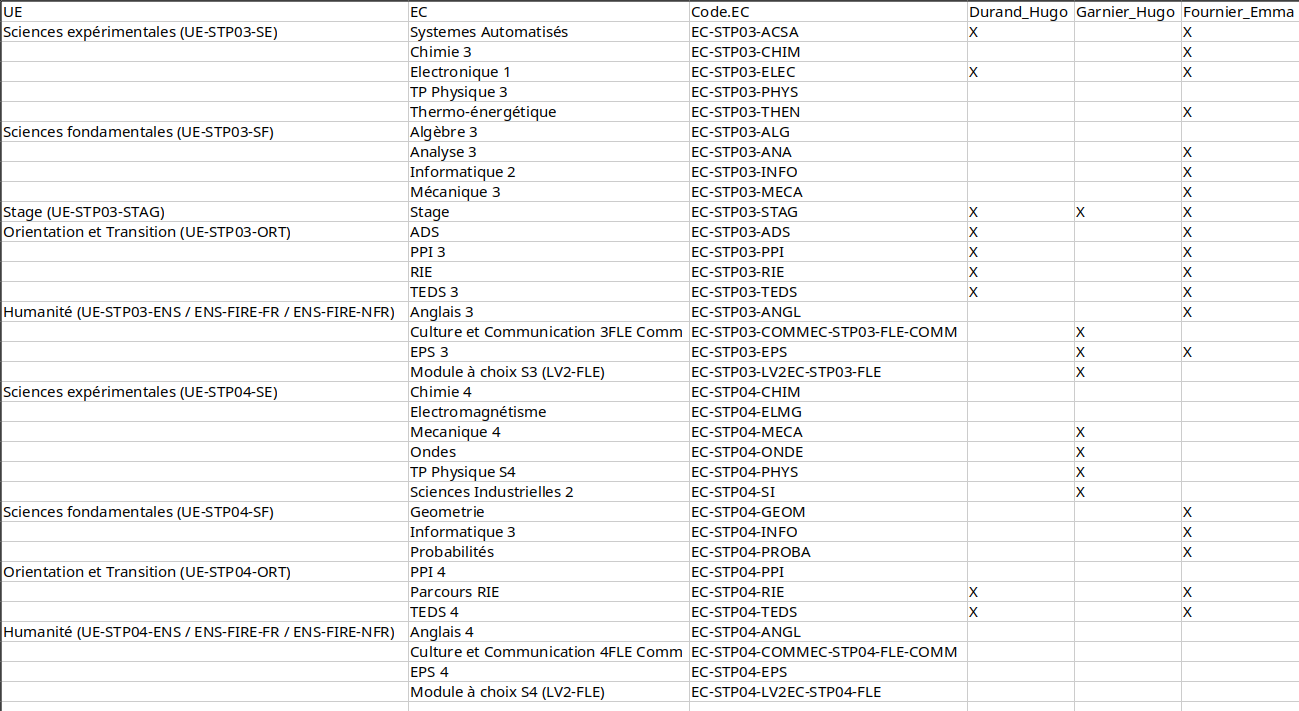
\includegraphics[width=\linewidth]{images/bilan.png}
  \caption{Extrait du bilan de l'ensemble de l'année}
  \label{generation_bilan}
\end{figure}

Ces bilans contiennent la liste des étudiants redoublants ainsi que les unités d’enseignement qu’ils devront repasser lors de la prochaine année universitaire. Ils constituent un outil précieux pour l’administration pédagogique dans le suivi des parcours étudiants.


\section{Bilan }
  \input{"bilan.tex"}

\section*{Conclusion}
TODO

\bibliography{BiblioEP}


\end{document}


